\setcounter{figure}{0} %reincia la numeración de las figuras
\renewcommand{\thefigure}{\thesection.\arabic{figure}}
\section{\Large Introducción}

\subsection{\large Motivación/Problemática del estudio}

       Indicar contexto de la tesis. Deben mencionarse las palabras claves, de lo que trata la tesis.\par
  
       Indicar antecedentes que guarden relación con la problemática de la tesis. Un contexto más específico.\par
       

       Si no quedó planteado en el párrafo anterior, en este párrafo debe plantearse la problemática. Usualmente va seguida de una conjunción tal como: Sin embargo, a pesar de esto, no obstante. A veces, algunos autores manifiestan la problemática de manera más explícita poniéndola como una pregunta entre signos de interrogación.\par
 
       Antecedentes específicos acerca de cómo otros autores han aportado en la resolución de dicho problema. Este párrafo también debe dar luces de la hipótesis del trabajo.\par

       Indicar cómo se abordará el problema; es decir, qué metodologías utilizará, qué datos nuevos presentará y qué tipo de análisis hará con ellos.

           
    \begin{figure}[h]
        \centering
        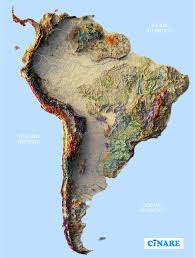
\includegraphics[width=0.3\linewidth]{images1.jpg}
        \caption{Mapa geológico regional de Sudamérica}
        \label{fig:mapareg}
    \end{figure}
            
\subsection{\large Hipótesis y Objetivos}
    
       En la hipótesis se debe indicar el modelo o posible solución al problema planteado y de qué manera los resultados que espera sostienen dicho modelo o solución. \par
     
       Se puede separar en Objetivo General o Principal y específicos o secundarios. \par
   
        En el objetivo principal se plantea de manera explícita que, a través de los resultados de este trabajo, se pretende resolver el problema planteado en la introducción o fortalecer un modelo que lo explique.\par
         
        En los objetivos específicos se debe indicar las etapas que deben cumplirse para lograr el objetivo general. Debe responder a la pregunta: \textbf{¿Para qué realizaré cada parte del trabajo?} Cada uno de los objetivos específicos debe apuntar a la resolución del objetivo general. Si no es así, significa que el objetivo específico no corresponde o que el objetivo general quedo mal planteado.

        
        \subsection{\large Metodologías}
Indicar los métodos que utilizará para llevar a cabo cada uno de los objetivos específicos que deben cumplirse para lograr el objetivo general. Debe responder a la pregunta: \textbf{¿Cómo realizaré cada parte del trabajo?} Cada una de las metodologías debe apuntar a la resolución de un objetivo específico. Si no es así, significa que la metodología no corresponde. A su vez, debe existir a lo menos una metodología que permita resolver cada objetivo específico, de lo contrario, la metodología no estaría completa.\par
            deberá escribirse la explicación detallada de los procedimientos seguidos e instrumental usado en las tareas de campo, laboratorio y gabinete.
     
        \subsection{\large Características del área de estudio}
            \subsubsection{Ubicación y acceso}
            Indicar vías de acceso y tipo de movilización que se requiere para acceder al área de estudio.
            \begin{figure} [h] %[h] fuerza a que la fig. se ubique en este lugar.
                \centering
                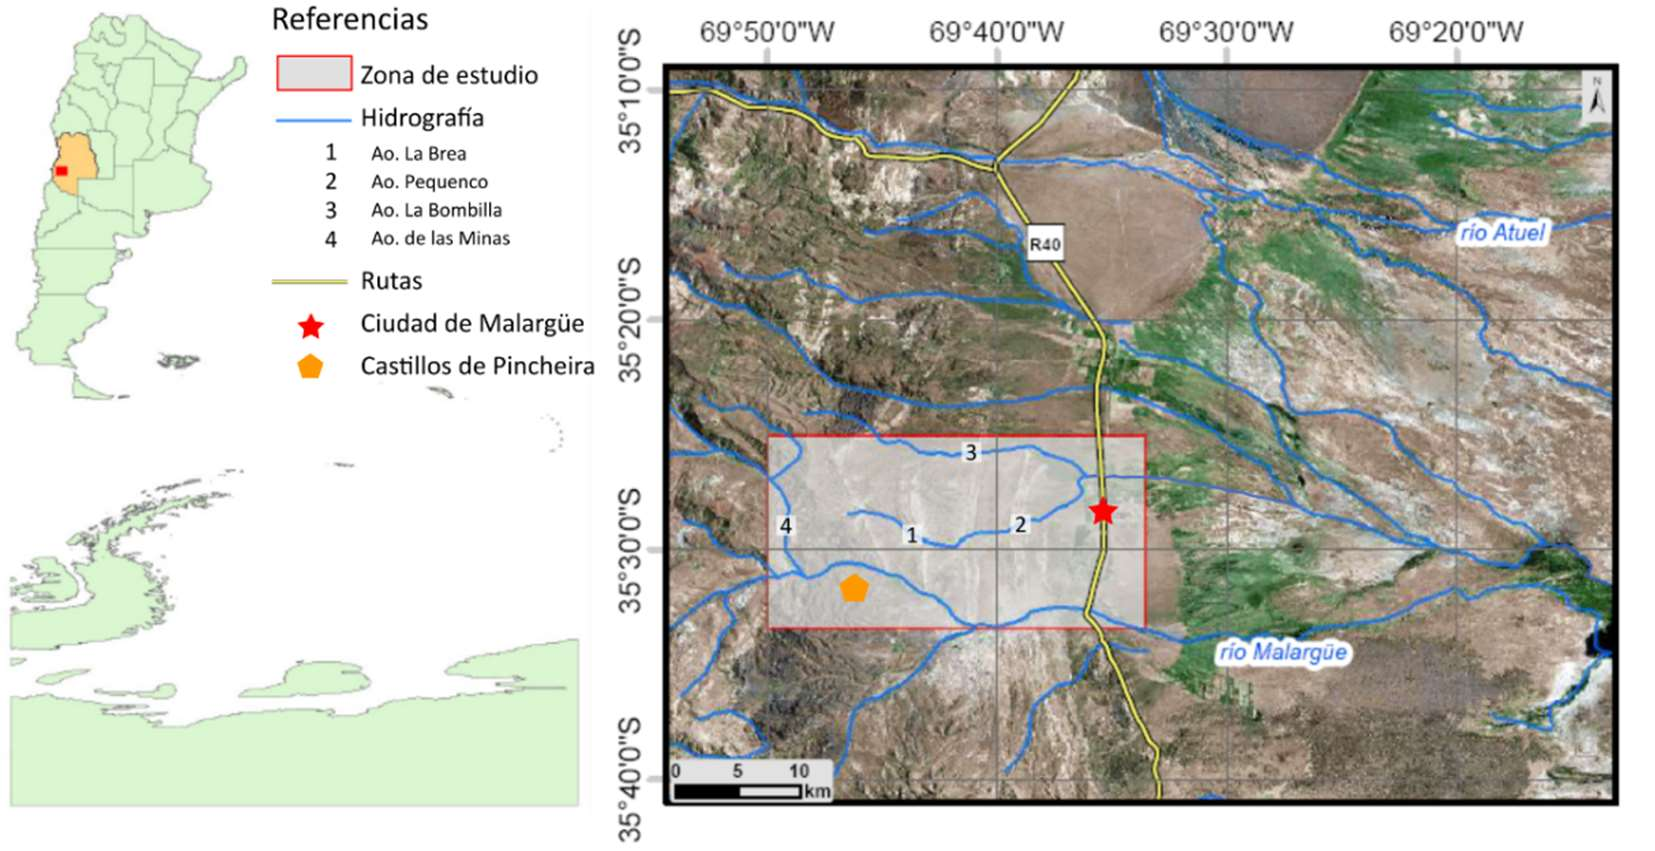
\includegraphics[width=0.7\linewidth]{Fig. ubicacion.jpg}
                \caption{\small Mapa de ubicación de la zona de estudio. En la imagen satelital de la derecha se marca con un rectangulo rojo el área de estudio.}
                \label{fig:enter-label}
            \end{figure}
            \subsubsection{Geografía}
             Se puede o no agregar esta subsección. Si se la considera entonces se deben agregar algunas características relevantes de la zona y que sean necesarias mencionar en el contexto de la tesis. 
            \subsubsection{Clima}
             Se puede o no agregar esta subsección. Si se la considera entonces se deben agregar algunas características relevantes de la zona y que sean necesarias mencionar en el contexto de la tesis. 
            \subsubsection{Hidrología}
            Se puede o no agregar esta subsección. Si se la considera entonces se deben agregar algunas características relevantes de la zona y que sean necesarias mencionar en el contexto de la tesis. 
            \subsubsection{Flora y Fauna}
            Se puede o no agregar esta subsección. Si se la considera entonces se deben agregar algunas características relevantes de la zona y que sean necesarias mencionar en el contexto de la tesis. 
        \subsection{\large Antecedentes}
            Se deben mencionar los principales trabajos previos que se realizaron en el área de estudio y los principales aportes de cada uno de ellos al conocimiento geológico del área de estudio. Hacer énfasis en los trabajos que abordaron temáticas o resultados que tienen que ver con la problemática de la tesis.